\documentclass[aspectratio=169]{beamer}
\usepackage[utf8]{inputenc}
\usepackage[english]{babel}
\usepackage{graphicx}
\usepackage{hyperref}
\usepackage{booktabs}
\usepackage{amsmath}

\usetheme{Madrid}
\usecolortheme{beaver}

\title{Lab 0: Machine Learning and PyCaret}
\subtitle{BMED365-2026: Computational Imaging, Modeling and AI in Biomedicine}
\author{BMED365}
\date{Spring 2026}

\begin{document}

\frame{\titlepage}

\begin{frame}{Overview}
    \tableofcontents
\end{frame}

\section{Introduction to Machine Learning}
\begin{frame}{What is Machine Learning (ML)?}
    \begin{columns}
        \column{0.6\textwidth}
        Machine learning is the study of computer algorithms that improve automatically through experience.
        
        \vspace{0.5cm}
        \textbf{Formal definition (Tom Mitchell):}
        A computer program is said to learn from experience \textbf{E} with respect to a task \textbf{T} and performance measure \textbf{P}, if its performance on T, as measured by P, improves with experience E.
        
        \vspace{0.5cm}
        \textit{In medicine:} 
        \begin{itemize}
            \item \textbf{T}: Diagnose a disease.
            \item \textbf{E}: Historical patient data.
            \item \textbf{P}: Accuracy.
        \end{itemize}
        
        \column{0.4\textwidth}
        \begin{block}{Prompt}
            \scriptsize\textit{"A clean, horizontal flowchart illustrating the machine learning pipeline on white background. Steps from left to right: 1) Raw data (database icon), 2) Preprocessing (gear), 3) Training (brain-chip icon), 4) Evaluation (magnifying glass on graph), 5) Deployment (cloud). Style is modern, 'Corporate Memphis' but strictly professional and medical-technical. High quality, vector style."}
        \end{block}
        \centering
        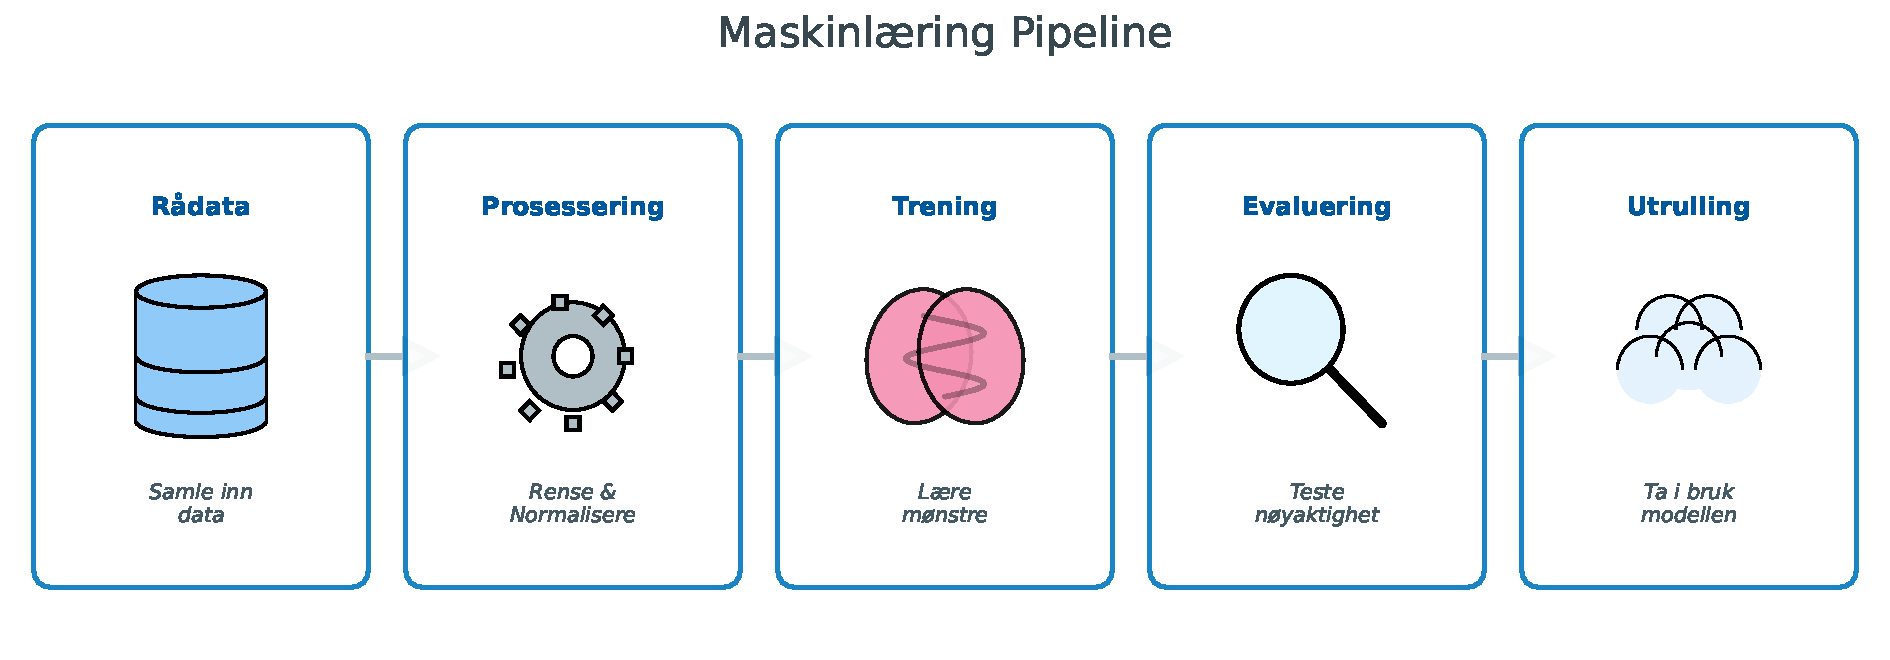
\includegraphics[width=0.9\textwidth]{images/ml_pipeline.pdf}
    \end{columns}
\end{frame}

\begin{frame}{ML Paradigms}
    \begin{itemize}
        \item \textbf{Supervised Learning:}
        We have input data $X$ and ground truth (labels) $y$. The goal is to learn a function $f: X \rightarrow y$.
        \begin{itemize}
            \item \textit{Classification:} $y$ is a category (Sick/Healthy).
            \item \textit{Regression:} $y$ is a continuous value (Blood pressure, Length of stay).
        \end{itemize}
        
        \item \textbf{Unsupervised Learning:}
        We only have input data $X$. The goal is to find structure in the data.
        \begin{itemize}
            \item \textit{Clustering:} Find patient groups.
            \item \textit{Dimensionality reduction:} Simplify complex data.
        \end{itemize}
    \end{itemize}
\end{frame}

\section{Classification vs. Regression}
\begin{frame}{Classification vs. Regression}
    \begin{columns}
        \column{0.5\textwidth}
        \textbf{Classification}
        \begin{itemize}
            \item Discrete output.
            \item E.g.: Diagnoses (ICD-10 codes).
            \item Algorithms: Logistic Regression, Decision Trees, Random Forest, SVM.
        \end{itemize}
        
        \column{0.5\textwidth}
        \textbf{Regression}
        \begin{itemize}
            \item Continuous output.
            \item E.g.: Time to event, dosage.
            \item Algorithms: Linear Regression, Random Forest Regressor, XGBoost.
        \end{itemize}
    \end{columns}
    
    \vspace{0.5cm}
    \begin{block}{Prompt}
        \scriptsize\textit{"Split screen scientific illustration. Left side labeled 'Classification': A scatter plot where a line separates red dots from blue dots. Right side labeled 'Regression': A scatter plot with a smooth curve fitting through the data points. Clean, white background, clear colors, high resolution, textbook quality."}
    \end{block}
    \centering
    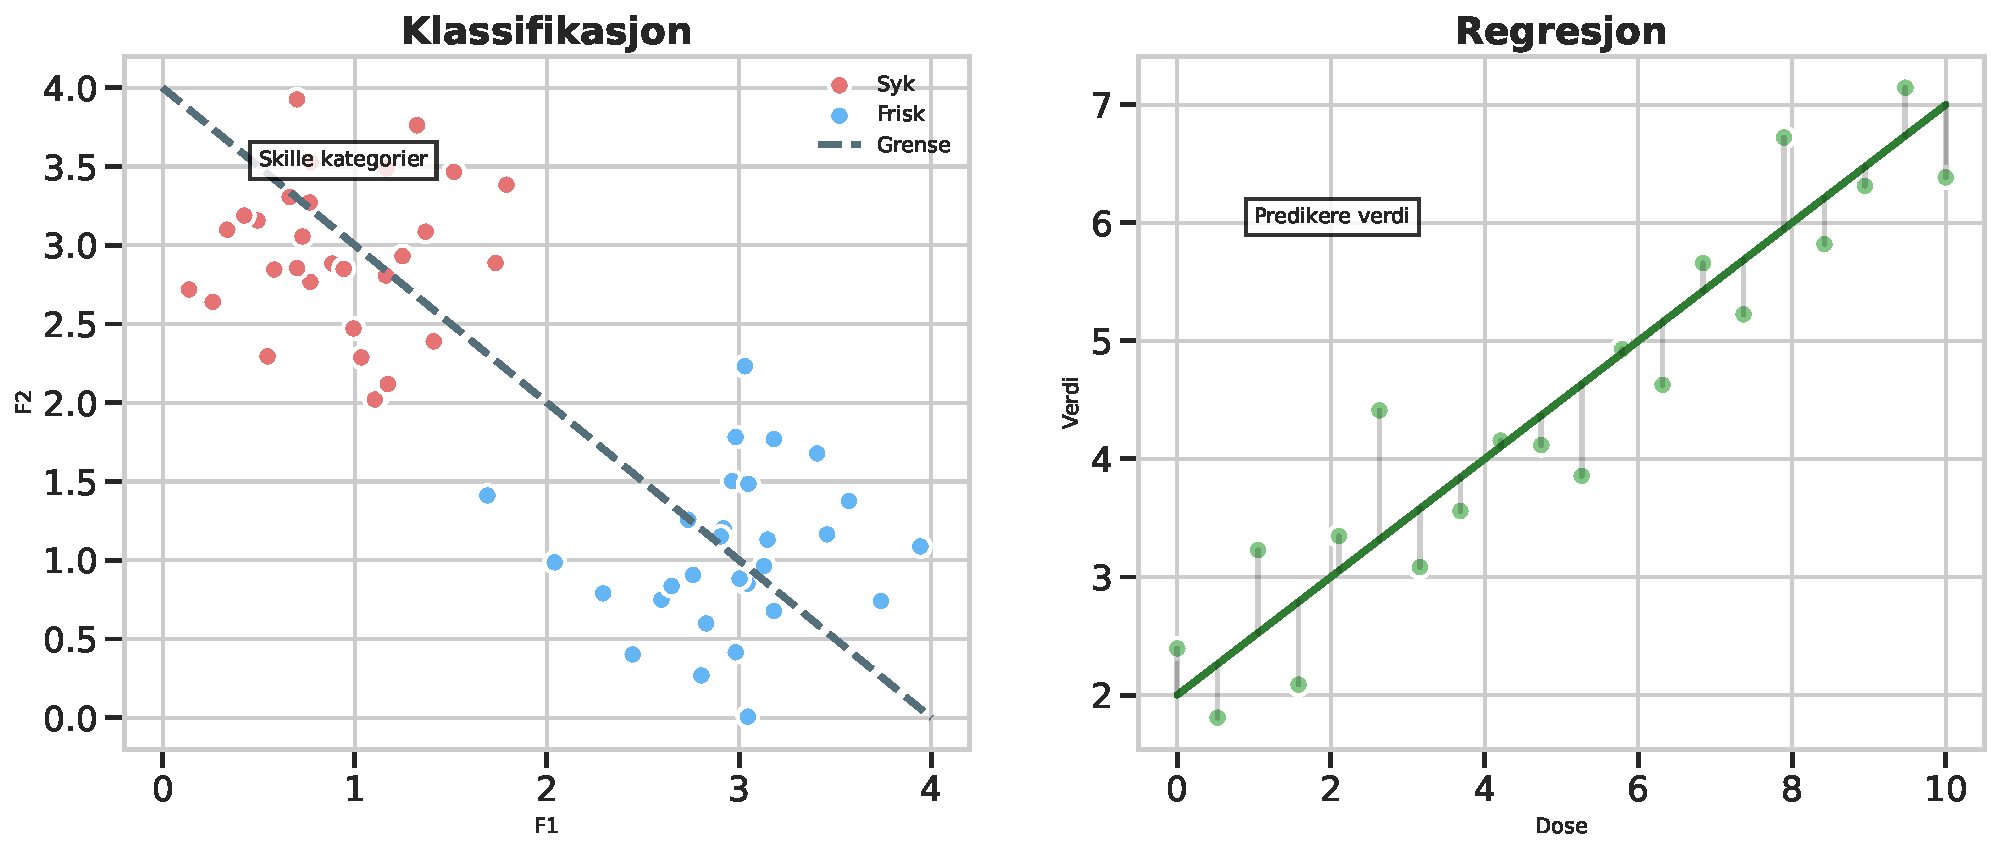
\includegraphics[width=0.7\textwidth]{images/class_vs_reg.pdf}
\end{frame}

\section{Model Evaluation}
\begin{frame}{How Do We Measure Success?}
    For classification we use a \textbf{Confusion Matrix}:
    
    \begin{table}[]
        \centering
        \begin{tabular}{|c|c|c|}
            \hline
             & \textbf{Predicted Positive} & \textbf{Predicted Negative} \\ \hline
            \textbf{Actual Positive} & True Positive (TP) & False Negative (FN) \\ \hline
            \textbf{Actual Negative} & False Positive (FP) & True Negative (TN) \\ \hline
        \end{tabular}
    \end{table}
    
    \vspace{0.2cm}
    \begin{itemize}
        \item \textbf{Accuracy:} $\frac{TP + TN}{Total}$ (Can be misleading with imbalanced data!)
        \item \textbf{Precision:} $\frac{TP}{TP + FP}$ (How many of those we called sick are actually sick?)
        \item \textbf{Recall (Sensitivity):} $\frac{TP}{TP + FN}$ (How many of the sick did we find?)
        \item \textbf{F1-Score:} Harmonic mean of Precision and Recall.
    \end{itemize}
\end{frame}

\begin{frame}{Bias-Variance Tradeoff}
    A central challenge in ML is the balance between \textit{bias} and \textit{variance}.
    
    \begin{columns}
        \column{0.5\textwidth}
        \textbf{Underfitting (High Bias):}
        \begin{itemize}
            \item The model is too simple.
            \item Does not capture the pattern in the data.
            \item Poor on both training and test.
        \end{itemize}
        
        \column{0.5\textwidth}
        \textbf{Overfitting (High Variance):}
        \begin{itemize}
            \item The model is too complex.
            \item Learns "noise" in the training data.
            \item Good on training, poor on test.
        \end{itemize}
    \end{columns}
    \vspace{0.5cm}
    \textit{The goal is to find the "sweet spot" that generalizes well to new data.}
\end{frame}

\section{PyCaret}
\begin{frame}{PyCaret: Automated ML}
    PyCaret is a "low-code" library that automates large parts of the ML workflow.
    
    \begin{itemize}
        \item \textbf{setup():} Initializes the environment, handles missing values, encodes categorical variables, splits data.
        \item \textbf{compare\_models():} Trains and evaluates many algorithms side-by-side.
        \item \textbf{create\_model():} Trains a specific model.
        \item \textbf{tune\_model():} Optimizes hyperparameters automatically.
        \item \textbf{plot\_model():} Generates standardized figures (ROC, Feature Importance).
    \end{itemize}
\end{frame}

\begin{frame}[fragile]{Example PyCaret Code}
    \begin{verbatim}
from pycaret.classification import *

# 1. Setup
exp = setup(data=diabetes_df, target='Class variable', session_id=123)

# 2. Compare models
best_model = compare_models()

# 3. Analyze
evaluate_model(best_model)

# 4. Predict
predictions = predict_model(best_model, data=new_data)
    \end{verbatim}
\end{frame}

\section{Notebooks and Exercises}
\begin{frame}{Overview of Lab 0 Notebooks}
    \begin{enumerate}
        \item \textbf{01-Simple\_examples.ipynb}:
        \begin{itemize}
            \item Manual implementation of simple ML concepts.
            \item Understand decision trees and logistic regression "under the hood".
        \end{itemize}
        
        \item \textbf{02-Binary\_classification.ipynb}:
        \begin{itemize}
            \item Classify the Pima Indians Diabetes dataset.
            \item Focus on data exploration (EDA) and model validation.
        \end{itemize}
        
        \item \textbf{03-PyCaret\_quickguide.ipynb}:
        \begin{itemize}
            \item Efficient ML workflow with PyCaret on the same dataset.
            \item Comparison of how much time you save!
        \end{itemize}
    \end{enumerate}
\end{frame}

\begin{frame}{Key Learning Points}
    \begin{itemize}
        \item \textbf{Data is most important:} "Garbage in, garbage out". Spend time understanding the data.
        \item \textbf{Validation:} Never trust training score alone. Use cross-validation or a hold-out test set.
        \item \textbf{Base rate:} Always check if the model beats a simple guess (e.g., "everyone is healthy").
        \item \textbf{Interpretability:} Sometimes a simple model (Linear Regression) is better than a complex one (Black Box) if we need to understand \textit{why}.
    \end{itemize}
\end{frame}

\begin{frame}{Summary}
    Today we have laid the foundation for the rest of the course.
    \begin{itemize}
        \item We have defined ML.
        \item We have looked at the difference between classification and regression.
        \item We have introduced PyCaret as a powerful tool.
    \end{itemize}
    
    In the next lab (Lab 1) we will look at how we can use \textbf{Network Science} to find patients that are similar to each other (PSN).
\end{frame}

\end{document}
